%% Cleaned Beamer file converted to Metropolis
\documentclass[english,aspectratio=169]{beamer}

% -------------------------------------------------
% Fonts and encoding
% -------------------------------------------------
\usepackage[T1]{fontenc}
\usepackage[latin9]{inputenc}
\usepackage{lmodern}
\renewcommand{\sfdefault}{lmss}
\renewcommand{\ttdefault}{lmtt}

% -------------------------------------------------
% Language and layout
% -------------------------------------------------
\usepackage{babel}
\setlength{\parskip}{\medskipamount}
\setlength{\parindent}{0pt}

% -------------------------------------------------
% Math, graphics, listings
% -------------------------------------------------
\usepackage{amssymb}
\usepackage{graphicx}
\usepackage{color}
\usepackage{tikz}
\usepackage{listings}
\renewcommand{\lstlistingname}{Listing}

% -------------------------------------------------
% Beamer configuration
% -------------------------------------------------
%\usetheme{CambridgeUS}

% -------------------------------------------------
% Theme: Metropolis
% -------------------------------------------------
\usetheme{metropolis}
\metroset{progressbar=frametitle,sectionpage=progressbar}

% -------------------------------------------------
% UCT Brand Colors
% -------------------------------------------------
\definecolor{UCTBlue}{HTML}{009ADA}
\definecolor{UCTDarkBlue}{HTML}{00243A}

\setbeamercolor{palette primary}{bg=UCTDarkBlue, fg=white}
\setbeamercolor{frametitle}{bg=UCTDarkBlue, fg=white}
\setbeamercolor{progress bar}{fg=UCTBlue}
\setbeamercolor{title separator}{fg=UCTBlue}
\setbeamercolor{alerted text}{fg=UCTBlue}

% -------------------------------------------------
% Custom UCT title slide
% -------------------------------------------------
\setbeamertemplate{title page}{%
  \begin{tikzpicture}[remember picture,overlay]
    % Background
    \fill[UCTBlue] (current page.south west) rectangle (current page.north east);
    % Logo
    \node[anchor=north, xshift=-4cm, yshift=-1.2cm] at (current page.north)
      {\includegraphics[height=1cm]{uct_logo_horizontal_white}};
    \node[anchor=north, xshift=4cm, yshift=0cm] at (current page.north)
      {
\includegraphics[height=3cm]{samos-logo-transparent}};      
  \end{tikzpicture}
  \vspace*{3.2cm}
  \begin{center}
    {\usebeamercolor[fg]{title}\usebeamerfont{title}\textcolor{white}{\inserttitle}}\\[0.6em]
    {\usebeamerfont{subtitle}\textcolor{white}{\insertsubtitle}}\\[1.2em]
    {\usebeamerfont{author}\textcolor{white}{\insertauthor}}\\[0.3em]
    {\usebeamerfont{institute}\textcolor{white}{\insertinstitute}}\\[0.8em]
    {\usebeamerfont{date}\textcolor{white}{\insertdate}}
  \end{center}
}

% -------------------------------------------------
% Footer logo for content slides
% -------------------------------------------------
\usepackage{tikzpagenodes}
\addtobeamertemplate{footline}{}{%
  \begin{tikzpicture}[remember picture,overlay]
    \node[anchor=south east, xshift=-1cm, yshift=0cm]
      at (current page.south east)
      {\includegraphics[height=0.5cm]{uct_logo_horizontal_blue}};
    \node[anchor=south west, xshift=0cm, yshift=-0.2cm]
      at (current page.south west)
      {
\includegraphics[height=0.7cm]{samos-logo-transparent.png}};  
  \end{tikzpicture}%
}

% -------------------------------------------------
% LyX-specific definitions (kept minimal)
% -------------------------------------------------
\makeatletter

\newcommand\makebeamertitle{\frame{\maketitle}}

\AtBeginDocument{%
  \let\origtableofcontents=\tableofcontents
  \def\tableofcontents{\@ifnextchar[{\origtableofcontents}{\gobbletableofcontents}}
  \def\gobbletableofcontents#1{\origtableofcontents}
}

\newenvironment{lyxcode}
  {\begin{list}{}{
     \setlength{\rightmargin}{\leftmargin}
     \setlength{\listparindent}{0pt}
     \setlength{\itemsep}{0pt}
     \setlength{\parsep}{0pt}
     \raggedright\normalfont\ttfamily
   }\item[]}
  {\end{list}}

\makeatother

% -------------------------------------------------
% Document
% -------------------------------------------------

\begin{document}
    \title[Core 3 ]{Day 1: Scientific Computing and Data Management}
    \author{Vichi and Mangatane}
    \institute[UCT]{Department of Oceanography\\marcello.vichi@uct.ac.za}
    \date{AOS-SAMOS}
    \maketitle

\begin{frame}{Outline}
    \tableofcontents{}
\end{frame}

% =================================================
\section{M: Introduction to SCDM (0.5 hour)}
% =================================================

\begin{frame}{Oceanography is an observational and computational science}

\begin{fact}
Ocean scientists collect data or access data collected by others
\end{fact}

\begin{itemize}
\item {\small{}Many scientists choose to work with a specific software for
data analysis and visualization but soon realize that much of the
work is not only writing computationally intensive number-crunching
loops}{\small\par}
\item {\small{}Very often programming is about }\textbf{\small{}shuffling
data in and out of different tools, converting one data format to another, extracting numerical data from a text, and administering experiments involving a large number of data files and directories}{\small{}.
(HP Langtangen, Python Scripting for Computational Science, 2008)}{\small\par}
\item This workflow must be properly organized, no matter which operating
system or software you have chosen
\end{itemize}
\end{frame}

% =================================================
\begin{frame}{The data<->science workflow}

The aim of this course is to increase the productivity of your data-to-science workflow, by presenting you with a few examples of methodologies and tools
\begin{enumerate}
\item Production/Collection \emph{(Investigation and Meta-search)}
\item Retrieval \emph{(Transfer)}
\item Data Management \emph{(Short-term archival and meta-data)}
\item Processing \emph{(Programming and Revision control)}
\item Analysis \emph{(Programming and Revision control)}
\item Publication or Higher Level Production \emph{(Programming, Revision
control and meta-data)}
\item Data Management \emph{(Long-term archival and meta-data)}
\end{enumerate}
\end{frame}

% =================================================
\begin{frame}{Data Management (DM)}

\framesubtitle{Adapted from the lecture notes by R. Roman and D. Byrne}

Data management comprises the following items:
\begin{itemize}
\item data collection
\item organisation
\item storage
\item preservation
\item publication
\end{itemize}
\end{frame}

% =================================================
\begin{frame}{Why do we need DM?}
\begin{itemize}
\item Government and research data, collected at public expense, must be properly managed in order to realize their full potential and justify their considerable production and maintenance costs
\item Your institution's and funding agency's expectations and policies
\item To ensure research integrity and validation of results.
\item To increase research efficiency
\item To facilitate data security and minimise the risk of data loss
\item To ensure wider dissemination and increased impact
\item To enable research continuity through secondary data use (permit new and innovative research to be built on existing information)
\item Uniqueness of observations => you cannot measure a 2001 temperature again!
\item Journals now request data to be made available online for the study to be validated (Retraction watch) \href{https://retractionwatch.com/}{https://retractionwatch.com/} 
\end{itemize}
\end{frame}

% =================================================
\begin{frame}{Preventing data loss}
\begin{columns}[t]

\column{6cm}
\begin{itemize}
\item - human error
\item - natural disaster
\item - facilities infrastructure failure
\item - storage failure
\item - server hardware/software failure
\item - application software failure
\end{itemize}

\column{6cm}
\begin{itemize}
\item - format obsolescence {[}floppy and stiffy drives{]}
\item - legal encumbrance
\item - malicious attack
\item - loss of staffing competencies
\item - loss of institutional commitment
\item - loss of financial stability
\end{itemize}
\end{columns}

\end{frame}

% =================================================
\begin{frame}{Principles of good DM}
\begin{itemize}
\item Define a research data management policy (University of Cape Town
data policy: \href{http://www.digitalservices.lib.uct.ac.za/dls/rdm-policy}{http://www.digitalservices.lib.uct.ac.za/dls/rdm-policy})
\item Data ownership (clear identification who has managerial and financial
control; legal rights along with copyright and intellectual property
rights)
\item Data documentation and metadata compilation {[}metadata applicable
to your field{]}
\item Data quality and standardisation
\item Data life-cycle control
\item Data custodian (not a person)
\item Data access and dissemination
\end{itemize}
\end{frame}

% =================================================
\begin{frame}{Definition: Research Data}

Research data is defined as \textbf{recorded factual material} commonly retained by and accepted in the scientific community as necessary to validate research findings \href{http://www.epsrc.ac.uk/about/standards/researchdata/scope}{http://www.epsrc.ac.uk/about/standards/researchdata/scope} 

Forms of research data
\begin{enumerate}
\item Observational (data captured in real-time: sensor data, survey data, sample data)
\item Experimental (data from lab equipment, often reproducible)
\item Simulations (data generated from models: climate and oceanic models)
\item Derived/compiled (data is reproducible, text and data mining)
\item Reference (collection of peer-reviewed datasets that are published
and curated)
\end{enumerate}
\end{frame}

% =================================================
\begin{frame}{Data Management Plans}
\begin{columns}[t]

\column{7cm}

Most of the data collected in Ocean Sciences will eventually become \textbf{digital data}. A DMP is always needed, and considerations must be done prior to collecting any data. 
\begin{itemize}
\item Types of data
\item Data sharing, access \& security, 
\item Metadata standards, 
\item re-use, archiving \& long-term preservation. 
\end{itemize}
Research data life cycle (Digital Curation Centre, \href{https://www.dcc.ac.uk}{www.dcc.ac.uk})

\column{6cm}

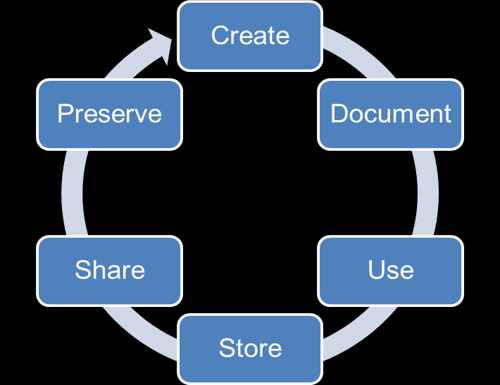
\includegraphics[width=6cm]{figures/DMP}
\end{columns}

\end{frame}

% =================================================
\begin{frame}{Data curation and visualization are recognized scholarly roles }
\begin{columns}[t]
\column{6cm}
\begin{itemize}
    \item Visualization - Preparation, creation and/or presentation of the published work, specifically visualization/data presentation.
    \item Data curation - Management activities to annotate (produce metadata), scrub data and maintain research data (including software code, where it is necessary for interpreting the data itself) for initial use and later re-use.
\end{itemize}
\column{6cm}


\includegraphics[width=6cm]{figures/credit.png}
\end{columns}

\end{frame}

% =================================================
\begin{frame}{Scripting and programming:\ the key to success}

\begin{columns}[t]

\column{7cm}

{\footnotesize{}\url{http://www.nature.com/naturejobs/science/articles/10.1038/nj7638-563a?WT.mc_id=FBK_NatureNews}}{\footnotesize\par}

{\footnotesize{}There are basically 3 choices to combine the computational capabilities of modern programming languages with processing and analysis of multidisciplinary ocean data}{\footnotesize\par}
\begin{itemize}
\item \emph{\footnotesize{}Matlab}{\footnotesize{} (commercial software, open-source version }\emph{\footnotesize{}octave}{\footnotesize{})}{\footnotesize\par}
\item \emph{\footnotesize{}R}{\footnotesize{} (open source)}{\footnotesize\par}
\item \emph{\footnotesize{}Python}{\footnotesize{} (open source)}{\footnotesize\par}
\end{itemize}
{\footnotesize{}They all have pros and cons and they are all interpreted scripting languages (more on this in
the next lectures), which will allow us to handle the typical data objects needed for ocean sciences}{\footnotesize\par}

\column{6cm}
\begin{itemize}
    \item {\footnotesize{}R and Python are the language of choice in this course, but we will also learn the multiple ways of interfacing with a computer and how to work with the filesystem.}
    \item {\footnotesize{}Datacamp will be used as the self-learning environment to guide you through the first steps with python}
    \item {\footnotesize{}on-line assignments will contribute to the final mark of the module }
    \end{itemize}
    \end{columns}

\end{frame}

% =================================================
\begin{frame}{Programming languages}
\begin{itemize}
  \item A programming language is a structured set of instructions that tells a computer what to do.
  \item Many languages have existed since the 1960s (e.g.\ FORTRAN), with some of them evolving over time (C to C++, C\#).
  \item Only a few dominate current general-purpose computing: Python, C++, Java, PHP.
  \item Why so many languages?
        \href{http://www.levenez.com/lang/}{levenez.com/lang}
\end{itemize}
\end{frame}

% -------------------------------------------------
\begin{frame}{High-level and low-level languages}
\begin{itemize}
  \item Python, R, FORTRAN, C++, PHP, C\#, Java are \textbf{high-level languages}.
  \item Computers only execute low-level (machine or assembly) languages.
  \item High-level programs must therefore be translated.
  \item Advantages:
    \begin{itemize}
      \item Easier to write, shorter, more readable
      \item More portable across systems
      \item Less error-prone
    \end{itemize}
  \item  
\end{itemize}
\end{frame}

% -------------------------------------------------
\begin{frame}{Interpreted and compiled languages}
\begin{itemize}
    \item Python and R are interpreted languages:
    \begin{itemize}
        \item an application interprets the language
        \item execute commands interactively with IDE (RStudio, jupyterlab, spyder)
        \item immediate feedback and easier debugging
    \end{itemize}
    \item FORTRAN, C++, etc. are compiled languages:
    \begin{itemize}
        \item code is written, compiled, and executed as a binary
        \item compilers allow optimization and portability to different OS
        \item debuggers are separate applications but IDEs are available to streamline workflow
    \end{itemize}
\end{itemize}
\end{frame}


% =================================================
\section{M: Hands-on tutorial - Jupyter Lab (1 hour)}
% =================================================
\begin{frame}{Hands-on tutorial}
    \begin{itemize}
    \item \textbf{\texttt{jupiterlab}}\\ an  Integrated Development Environment (IDE) for python notebooks \\(Sec. 3.4.2 on Amathuba)
    \item Objective: refresh some major features of \texttt{numpy} and learn how to use notebooks
    \end{itemize}
     
\end{frame}

% =================================================
\section{M: The computer interface - operating systems and filesystems (1.5 hour)}
% =================================================
\begin{frame}{The computer interface}
\begin{itemize}
\item The ``computer'' is a logical processing unit that must be instructed to perform operations (programmed)
\item It deals with information in a \textbf{digital} format, using electrical signals that are temporarily stored in a physical space called memory
\item The ``inventors'' of the computer \emph{idea} (Turing and von Neumann) created the mathematical methods to perform operations (programs) and to solve an \emph{infinite} set of problems. This developed the concept of the \textbf{Central Processing Unit} of programmable computers 
\item This was the first giant leap: what was needed was creating the technical possibility to translate the operations in a machine language and to return the results in a human-understandable language. The first working programmable computer was designed by Konrad Zuse in 1941. 
\item How do we interface with a contemporary computer?
\end{itemize}
\end{frame}

% =================================================
\begin{frame}{The operating system (OS)}

\begin{columns}[t]
\column{5cm}
\begin{itemize}
\item {\footnotesize{}The operating system is the agent that allows the
interaction between hardware (the components), software (the programmes) and the user \url{http://faculty.salina.k-state.edu/tim/ossg/Introduction/OSrole.html}}{\footnotesize\par}
\end{itemize}

\column{8cm}

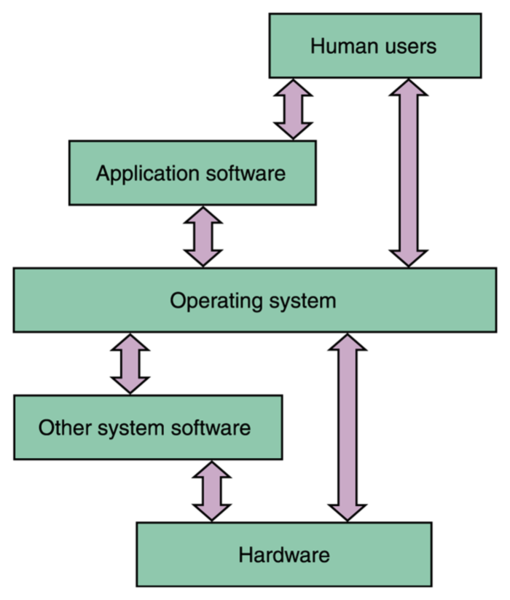
\includegraphics[width=6cm]{figures/OS_define}
\end{columns}

\end{frame}

% =================================================
\begin{frame}{What the OS does}

{\small{}The operating system is the }\textbf{\small{}software}{\small{}
}\textbf{\small{}interface}{\small{} that appears after the boot has completed, and runs underneath all other programs - without it nothing would happen at all. In simple terms, an operating system is a manager.
It manages all available resources on a computer, from the CPU, to memory, to network and hard disk accesses.}{\small\par}

{\small{}Tasks the operating system must perform:}{\small\par}
\begin{itemize}
\item {\small{}Control Hardware - The operating system controls all the
parts of the computer and attempts to get everything working together. }{\small\par}
\item {\small{}Run Applications - Another job the OS does is run application software. This would include word processors, web browsers, games,
etc... }{\small\par}
\item {\small{}Manage Data and Files - The OS makes it easy for you to organize your computer. Through the OS you are able to do a number of things to your data, including copy, move, delete, and rename them. This makes it much easier to find and organize what you have}{\small\par}
\end{itemize}
\end{frame}

% =================================================
\begin{frame}{Types of OS}
\begin{itemize}
\item Windows (originally DOS)
\item Mac OSX (based on UNIX)
\item UNIX and Linux
\item Android and iOS
\item Virtual OS: host and guest (VirtualBox, VMware, etc)
\end{itemize}
\end{frame}

% =================================================
\begin{frame}{Structure of an operating system}
\begin{columns}[c]
\column{6cm}
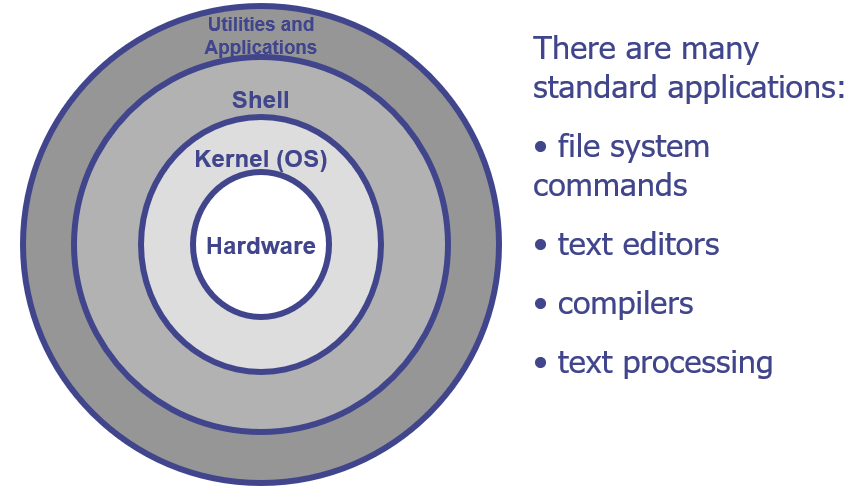
\includegraphics[width=7cm]{figures/unix_structure}
\begin{itemize}
\item \scriptsize{\textbf{Kernel or OS} -- It handles memory management, input and output requests, and program scheduling. It provides the basic software connection to the hardware. }
\end{itemize}

\column{8cm}
\begin{itemize}
\item \scriptsize{\textbf{Graphical User Interface (GUI) and shells} -- The GUI allows the user to perform gestures using graphical objects (buttons, menus, etc) to move files or launch applications. The shell sits behind the GUI; it is a program that provides a command line interface where the user must type literal commands. Gestures in the GUI are translated by the shell into something the kernel can comprehend, and then executed by the kernel.}
\item \scriptsize{\textbf{The Built-in System Utilities} -- are programs that allow a user to perform tasks which involve complex actions. Utilities provide user interface functions that are basic to an operating system, but
are too complex to be built into the shell. Examples of utilities are programs that let us see the contents of a directory, move \& copy files, remove files, etc... }
\item \scriptsize{\textbf{Application Software \& Utilities} -- these are not part of the operating system. They are additional programs that are bundled with the OS distribution, or installed by the user.}
\end{itemize}
\end{columns}

\end{frame}

% =================================================
\begin{frame}{Knowing the shell}

\begin{itemize}
\item All operating systems have a command line interface. The commands are typed by the user and executed by pressing the Enter key.  
\begin{itemize}
    \item Windows: Power Shell
    \item MacOS/Linux: Terminal 
\end{itemize}
\item Type the command \texttt{ls} and press Enter.
\item Type the command \texttt{pwd} and press Enter.
\item What do you see?
\end{itemize}

\end{frame}

% =================================================
\begin{frame}{Giving instructions to the OS: shell commands}

Commercial software is often insufficient to perform all the data processing operations needed in ocean sciences. We often have to 
\begin{itemize}
\item download bulk data from repositories (often at specific time intervals, e.g. every day)
\item perform the same operation on different files (temporal and spatial averages, extractions, etc.)
\item rename, cut, concatenate files, and convert between different formats
\end{itemize}
These operations require more than a GUI. This is where the shell (the language of the operating system) becomes relevant because it allows you to run batch operations (\emph{multiple commands that can be sequentially executed by the computer, often in the background}). You can run OS commands with all scientific computing languages.
\end{frame}


% =================================================
\begin{frame}[fragile]{Example of shell commands: Adding a UNIX terminal to Jupyter Lab}

Firstly, we will need to add some features to our Anaconda environment. Open the Anaconda prompt and type (followed by Enter) 
\begin{lyxcode}
    conda install git jupyterlab\_git
\end{lyxcode}

When finished, we need to adjust the Jupyter lab configuration. In the Anaconda Prompt, type the first command below, and press Enter, to generate the configuration file. The prompt will display the path where the file was created. We will \textit{edit} this file using the program \texttt{nano} in the terminal and add a new configuration setting to open a different terminal (\texttt{bash}).
\begin{lstlisting}[basicstyle=\scriptsize\ttfamily]
> jupyter lab --generate-config
Windows: C:\Users<YourUsername>\.jupyter\jupyter_lab_config.py
Mac/Linux: ~/.jupyter/jupyter_lab_config.py 

> nano jupyter_lab_config.py
c.ServerApp.terminado_settings = {'shell_command':['bash.exe']}
\end{lstlisting}

\end{frame}

% =================================================
\begin{frame}[fragile]{Tutorial: Bash shell in Jupyter Lab}
\begin{itemize}
    \item First download from Amathuba the \texttt{shell-lesson-data.zip} file and decompress it in your Download folder.
    \item From the same Anaconda Prompt window, we can also launch the application without using the Navigator: \texttt{> jupyter lab} (enter)
    \item launch the terminal from Jupyter Lab and test the following commands:
\end{itemize}

\begin{lstlisting}[basicstyle=\small\ttfamily]
> pwd
> cd Downloads/shell-lesson-data
> ls
> alias ls='ls --color'
> ls
\end{lstlisting}

\end{frame}

% -------------------------------------------------
\begin{frame}{The shell and the home directory}
\begin{itemize}
  \item The shell is an interpreted environment for interacting with the filesystem. You can do the same operations you do interactively with windows and folders.
  \item Your personal directory is called \emph{home}.
\end{itemize}

\begin{lyxcode}
/home/marcello
/c/Users/yourname
\end{lyxcode}

\begin{itemize}
  \item Files are stored in subdirectories under home. The command \texttt{cd 'dirname'} (change directory to 'dirname') allows you to navigate into children directories and back to the parent directory \texttt{cd ../}
  \item Use \texttt{cd} with no arguments to return home from anywhere.
\end{itemize}
\end{frame}

% -------------------------------------------------
\begin{frame}{The filesystem structure}
\centering
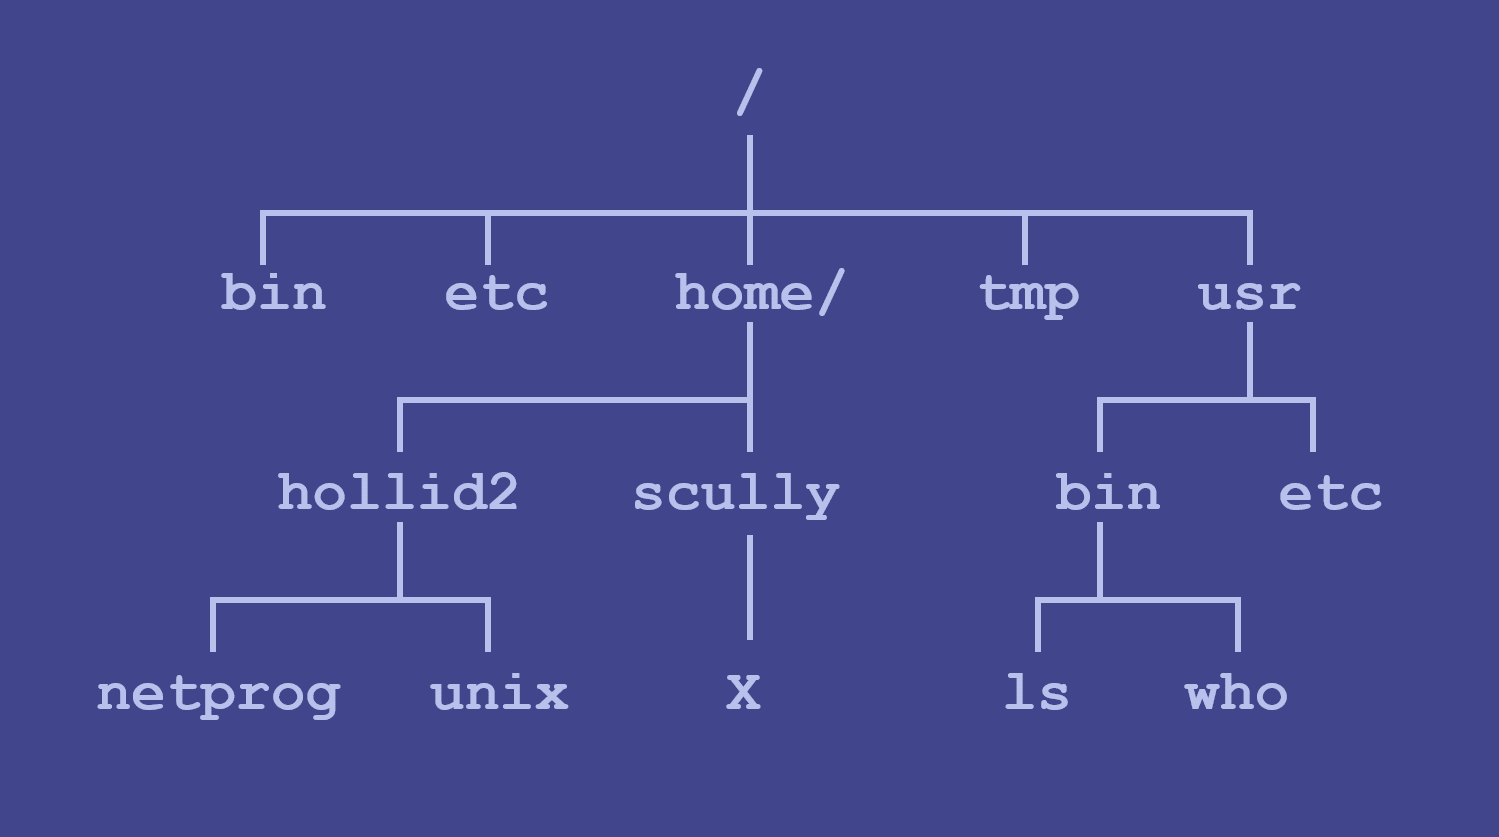
\includegraphics[width=7cm]{figures/unix_filesystem.png}

\begin{itemize}
  \item File names are case-sensitive.
  \item Directories are special files.
  \item The filesystem is hierarchical, rooted at \texttt{/}.
\end{itemize}
\end{frame}

% -------------------------------------------------
\begin{frame}{The pathname}
\begin{columns}
\column{6cm}
    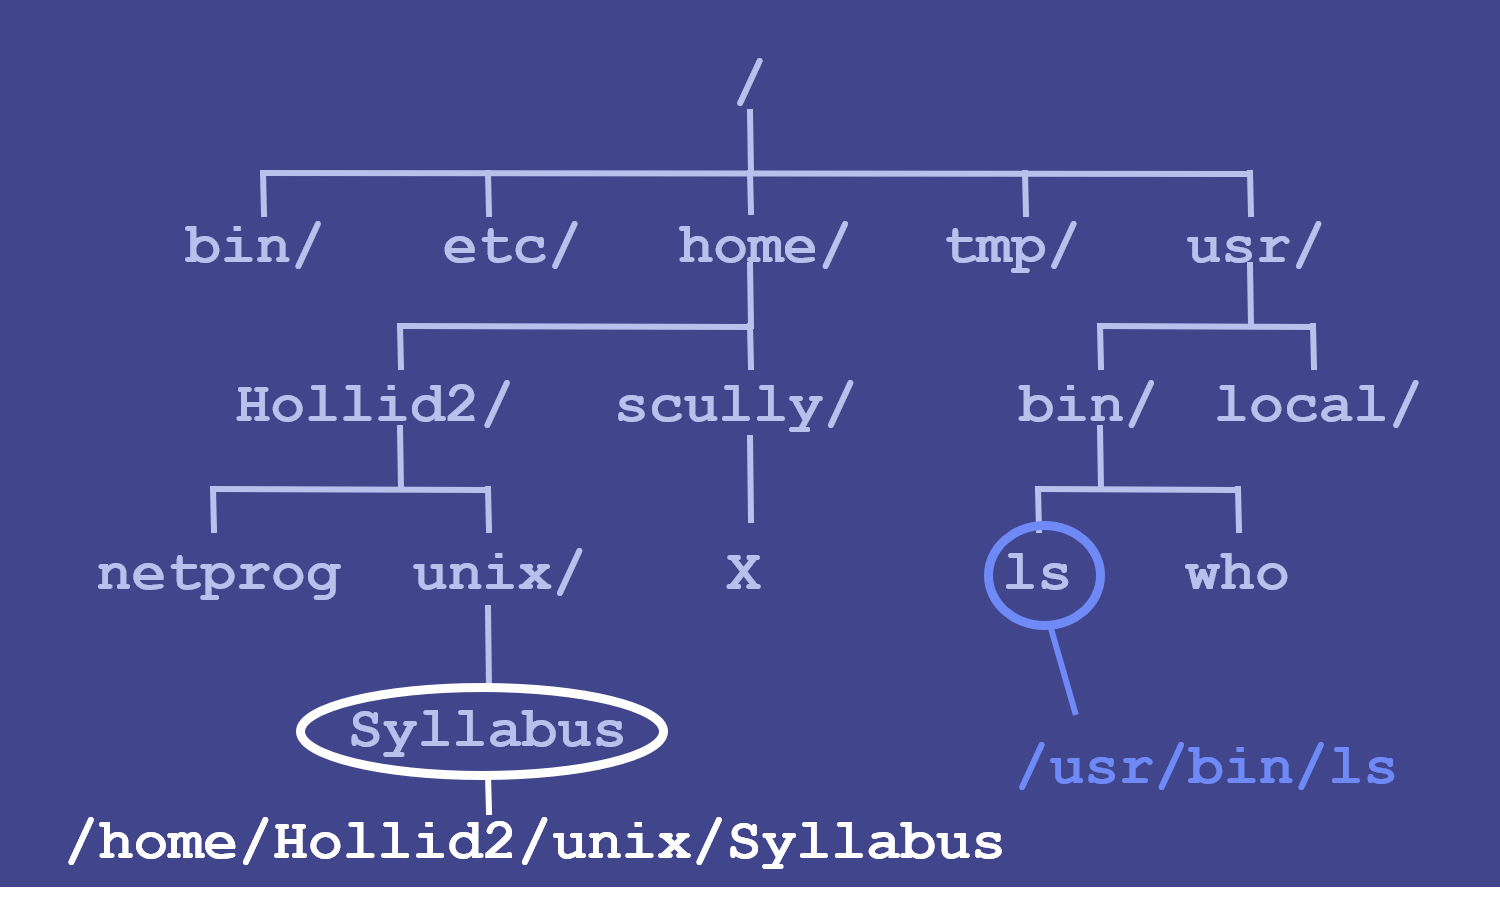
\includegraphics[width=6cm]{figures/unix_pathnames}

\column{7cm}
    \begin{itemize}
      \item A pathname uniquely identifies a file or a directory.
      \item You can use an absolute path as in the figure for file \texttt{Syllabus}.
      \item or you can use relative pathnames, e.g. from directory \texttt{unix} to file \texttt{ls}:
        \texttt{../../../usr/bin/ls}
          \item Practice (optional):
    \href{http://swcarpentry.github.io/shell-novice/}{Software Carpentry Shell}
    \end{itemize}
    \end{columns}
\end{frame}

% =================================================
\section{A: Programming and data\\(1.5 hour)}
% =================================================
\begin{frame}{Structures of a program}

\begin{columns}
\column{8cm}
\begin{itemize}
\item {\footnotesize{}Big codes are divided in smaller portions to improve usability and readability. They have a }\textbf{\footnotesize{}main
program}{\footnotesize{} and }\textbf{\footnotesize{}(sub)procedures}{\footnotesize\par}
\item {\footnotesize{}Procedures may be }
\begin{itemize}
\item \textbf{\footnotesize{}subroutines}{\footnotesize{} smaller portions of the code that do certain things and can be called with specific arguments. They are used to structure the code in meaningful self-contained
parts. Both the input and output arguments can be complex objects with multiple information}{\footnotesize\par}
\item \textbf{\footnotesize{}functions}{\footnotesize{} these are portions of the code that return }\emph{\footnotesize{}at least}{\footnotesize{}
one result. They are meant to be used many times, as for instance the intrinsic mathematical functions (}\texttt{\footnotesize{}sin,
cos, sqrt}{\footnotesize{}, etc.)}{\footnotesize\par}
\end{itemize}
\end{itemize}

\column{4cm}
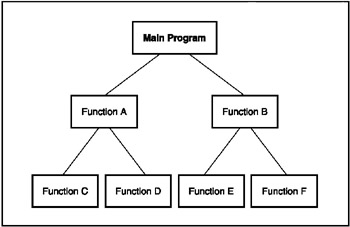
\includegraphics[width=4cm]{figures/functions}
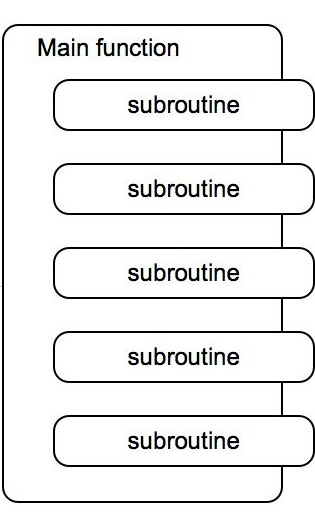
\includegraphics[width=3cm]{figures/subroutine}
\end{columns}

\end{frame}

% -------------------------------------------------
\begin{frame}{Structured programming (Wikipedia)}

\begin{center}
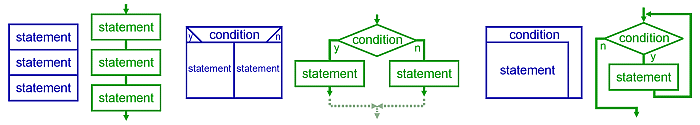
\includegraphics[scale=0.5]{figures/Structured_program_patterns}
\par\end{center}
\begin{description}
\item [{{\footnotesize{}Sequence}}] {\footnotesize{}ordered statements
or subroutines executed in sequence}{\footnotesize\par}
\item [{{\footnotesize{}Selection}}] {\footnotesize{}one or a number of statements is executed depending on the state of the program}\texttt{\footnotesize{}
if..then..else..endif}{\footnotesize{}.}{\footnotesize\par}
\item [{{\footnotesize{}Iteration}}] {\footnotesize{}a statement or block is executed until the program reaches a certain state, or operations have been applied to every element of a collection. This is usually expressed with keywords such as }\texttt{\footnotesize{}while, repeat,
for or do..until}{\footnotesize{}. }{\footnotesize\par}
\item [{{\footnotesize{}Recursion}}] {\footnotesize{}a statement is executed by repeatedly calling itself until termination conditions are met. }{\footnotesize\par}
\end{description}
\end{frame}

% -------------------------------------------------
\begin{frame}{Algorithms}

\begin{definition}
An algorithm is a specific set of instructions for carrying out a
procedure or solving a problem, usually with the requirement that the procedure terminate at some point \emph{(http://mathworld.wolfram.com/Algorithm.html) }
\end{definition}
\begin{itemize}
\item The word \textquotedbl algorithm\textquotedbl{} is a distortion of al-Khw\={a}rizm\={\i}, a Persian mathematician who wrote an influential
treatise about algebraic methods
\item The process of applying an algorithm to an input to obtain an output is called a computation
\item Algorithms are presented as flow charts and usually expressed in meta-language terms
\item This is done because they have to be generic and independent of the specific programming language
\end{itemize}
\end{frame}

% -------------------------------------------------
\begin{frame}{Flow charts}

\begin{columns}
\column{6cm}
\begin{itemize}
\item A flowchart is a graphical representation of an algorithm
\item It uses frame symbols to indicate certain basic operations (simple algebraic, input/output, decision making, etc.)
\item Symbols are connected to each other with arrows showing the flow and the meta-language operations are indicated inside the frame
\end{itemize}

\column{6cm}
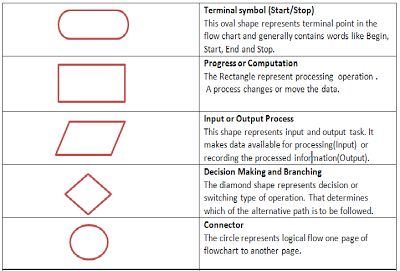
\includegraphics[width=6cm]{figures/flowchart_symbols}
\end{columns}

\end{frame}

% -------------------------------------------------
\begin{frame}[fragile]{A trivial example}

\begin{columns}
\column{6cm}
\begin{lstlisting}[basicstyle={\footnotesize\ttfamily},frame=shadowbox]
Meta-language Algorithm

Step 1: Start
Step 2: Input the values of 
        A and B
Step 3: Check if a>b,  
        - if yes then print 
          "A is maximum"
        - if no then print 
          "B is maximum"
Step 4: Stop
\end{lstlisting}

\column{6cm}
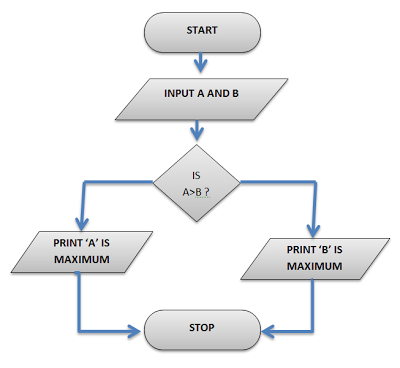
\includegraphics[width=6cm]{figures/flowchart_stupid}
\end{columns}
\end{frame}

% -------------------------------------------------
\begin{frame}{Another one with structured programming: Cooking a toast...}
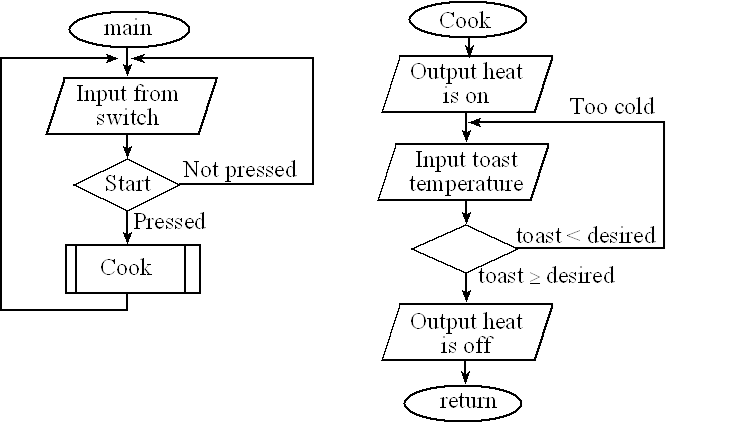
\includegraphics{figures/toast_cooking}
\end{frame}

% -------------------------------------------------
\begin{frame}{Basic digital data types}
\begin{itemize}
    \item {\small{}All machine-readable data are digital, which means that they are made of coded }\textbf{\small{}discrete}{\small{} information}
    \item {\small{}Data must have a format to be understood by the operating system }{\small\par}
    \begin{itemize}
    \item \textbf{\small{}Binary data}{\small{}: contain the bits and bytes of the information without a specific coding, and can be interpreted by a software that already knows what to look for.}
    \item \textbf{\small{}ASCII data}{\small{}: American Standard Code for Information Interchange. An ASCII code is the numerical representation of a character,
    which is still written in binary code but software knows how to handle the coding. 01101000 and 01101001 are equal to the decimal numbers 104 and 105, which in ASCII correspond to the letters \textquotedbl hi\textquotedbl}
    \end{itemize}
    \item {\small{}A text produced with MS Word is a binary file, even if it contains ASCII characters because it includes formatting information on how the document looks like. Text produced with a
    }\emph{\small{}text editor}{\small{} (e.g. notepad) is instead an ASCII file (called a }\textbf{\small{}flat file}{\small{}).}{\small\par}
    \item {\small{}A MS Excel ``table'' is not a flat file; only if you save it in ASCII format (e.g. using the Comma Separated Values format, CSV) it will be accessible by other ASCII applications.}{\small\par}
\end{itemize}
\end{frame}


% =================================================
\begin{frame}{Data transfer and protocols}
\begin{columns}[t]

\column{8cm}
\begin{itemize}
\item {\small{}Data must be on a support that is readable through a peripheral. Nowadays, we use files on }\emph{\small{}drives}{\small{} or through
the network. Originally (until the late 70's), the data were passed through paper, the }\textbf{\small{}punch cards}{\small{}, then through magnetic }\emph{\small{}floppy}{\small{} disks}{\small\par}
\item {\small{}On the Internet, data needs to be transferred in a coded way. These methods are called protocols}{\small\par}
\begin{itemize}
\item \textbf{\small{}HTTP}{\small{}(S): hyper text transfer protocol (the main protocol of browsers, written in HTML)}{\small\par}
\item \textbf{\small{}FTP}{\small{}: file transfer protocol (needs a terminal or apps)}{\small\par}
\end{itemize}
\end{itemize}

\column{6cm}

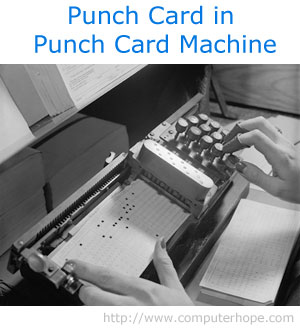
\includegraphics[width=4cm]{figures/punchcard}

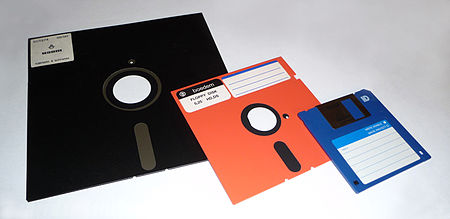
\includegraphics[width=6cm]{figures/450px-Floppy_disk_2009_G1}
\end{columns}

\end{frame}

% =================================================
\begin{frame}{Transfer and Storage: Apps or command line?}
\begin{columns}[t]

\column{4cm}
\begin{itemize}
\item {\tiny{}Data (file) transfer must be handled by specific applications
that know how to work with the protocols}{\tiny\par}
\item {\tiny{}This can be done through browsers, clients and command line applications}{\tiny\par}
\item {\tiny{}Several public data archive allows to access their data via several methods and for most of them it is possible to click on the data we want}{\tiny\par}
\item {\tiny{}But what if we want more than one data file? We need to use an application that allows this }\textbf{\tiny{}batch}{\tiny{} handling
or to write scripts for bulk download }{\tiny\par}
\end{itemize}

\column{8cm}

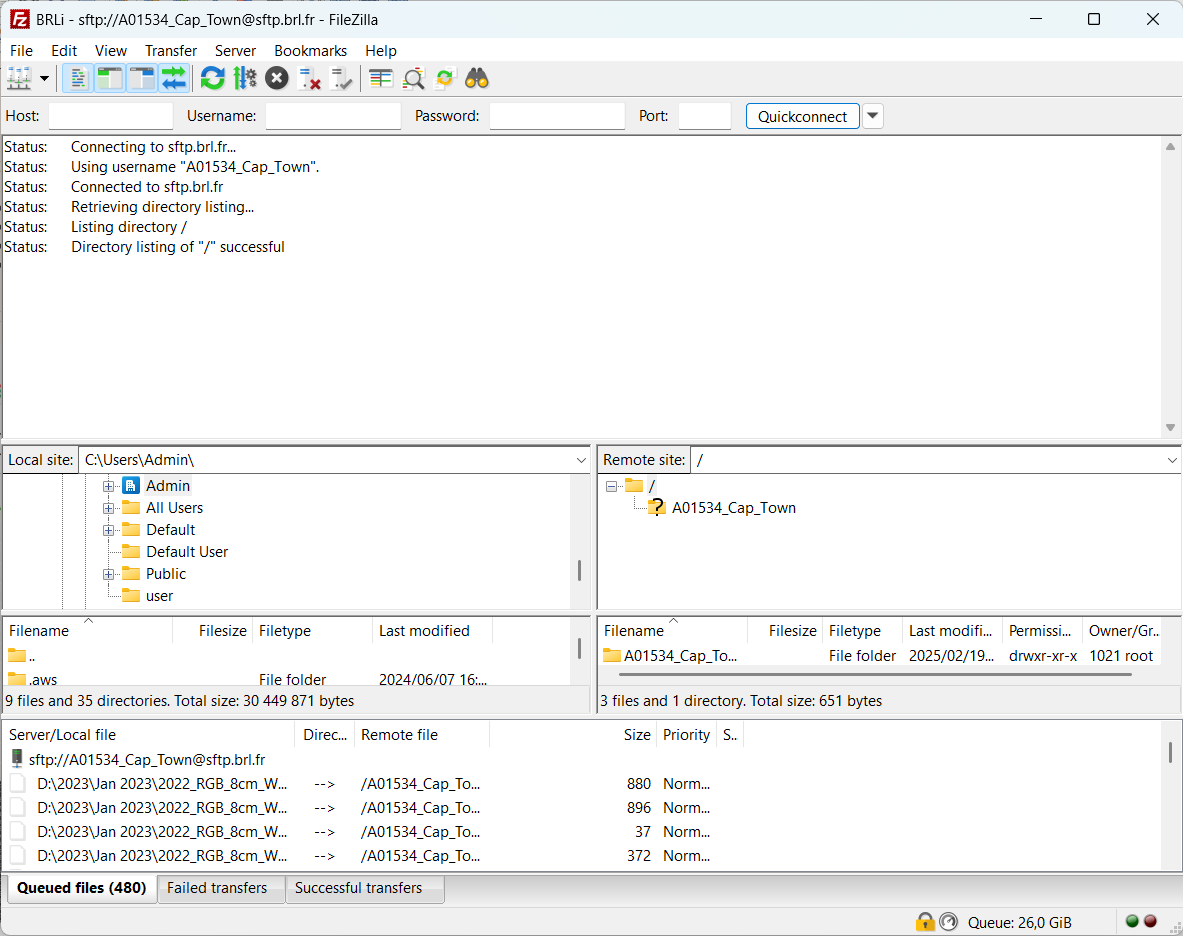
\includegraphics[width=3cm]{figures/ftp-browser}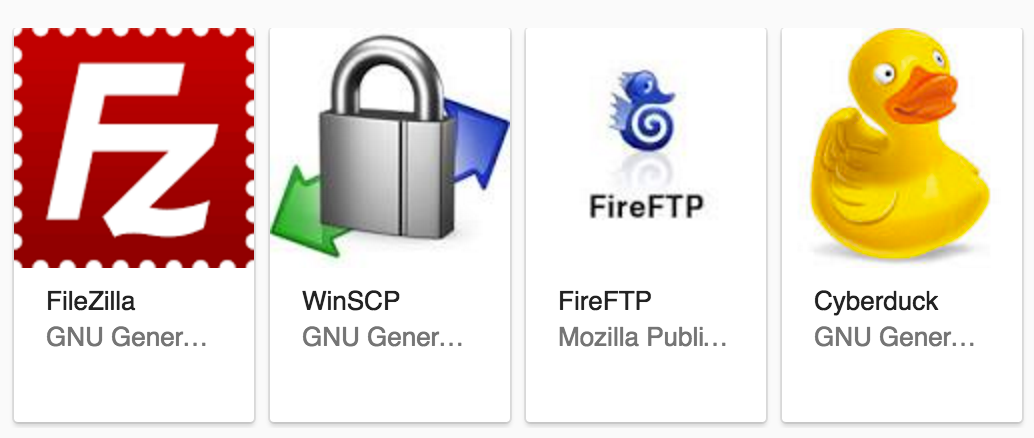
\includegraphics[width=4cm]{figures/ftp-clients}

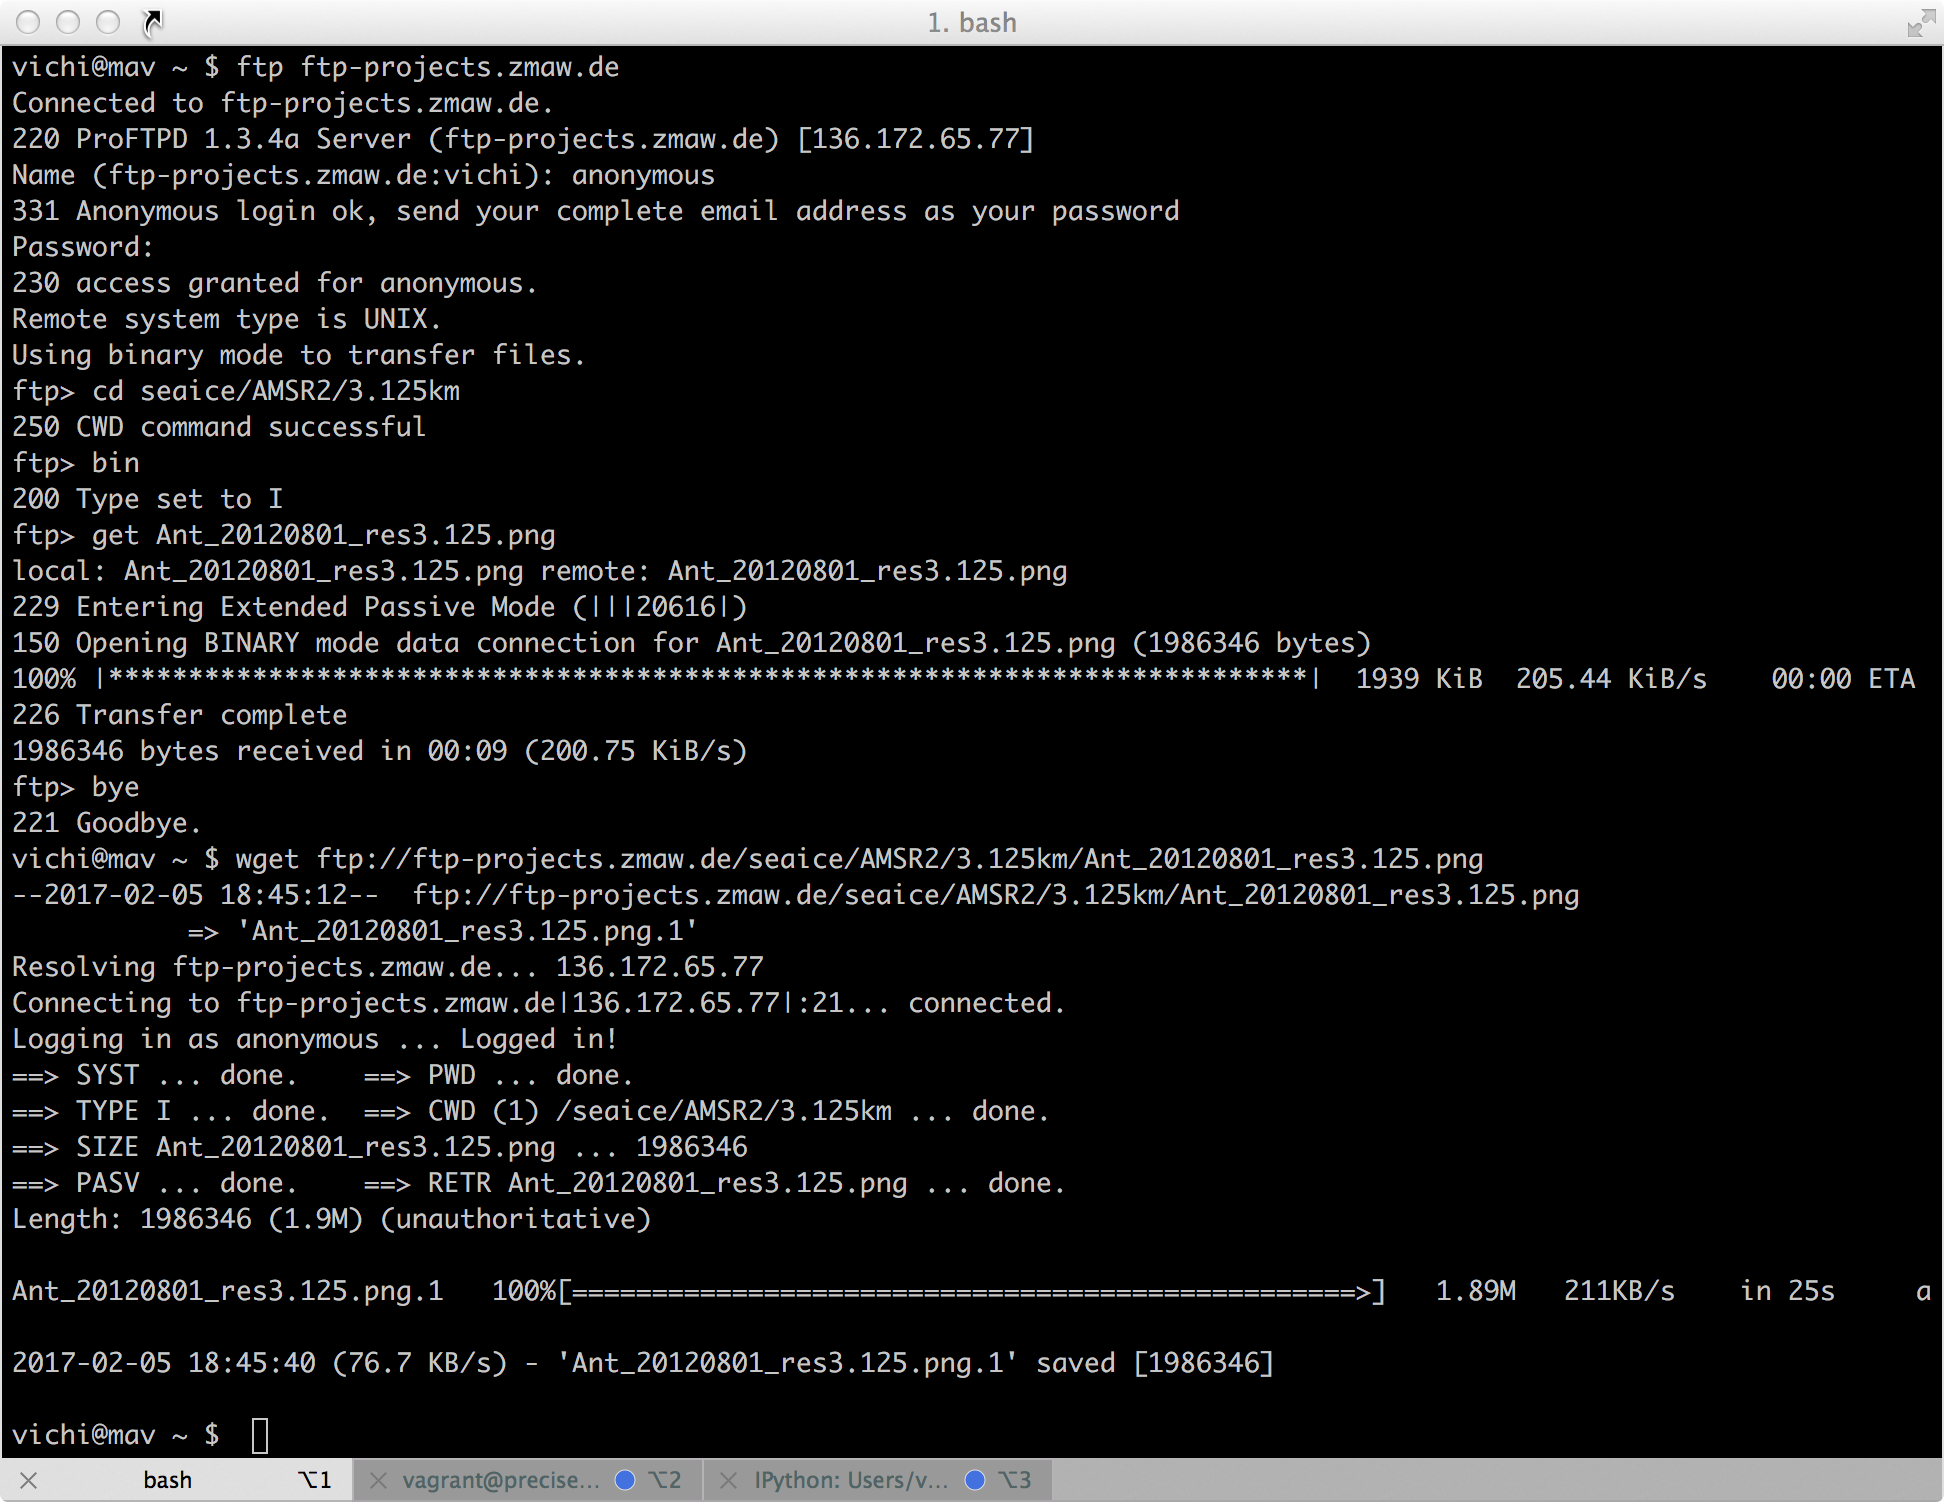
\includegraphics[width=8cm]{figures/ftp-command}
\end{columns}

\end{frame}

\begin{frame}{Hands-on tutorial}
    \begin{itemize}
    \item A batch python script to download daily sea ice concentration data from a public repository \href{https://seaice.uni-bremen.de/databrowser/#p=sic}{Sea Ice remote sensing - University of Bremen}
    \item Objective: compare the efficiency of using batch scripts against the click-download method
    \item We will use the command \texttt{curl}. Usage: \begin{lyxcode}
        curl -o fname URL
    \end{lyxcode}
    \end{itemize}
     
\end{frame}

% -------------------------------------------------
\begin{frame}[fragile]{Tutorial: your first batch download notebook}
\begin{lstlisting}[language=python,basicstyle=\tiny\ttfamily]
# Modules
import subprocess
from datetime import datetime, timedelta
from pathlib import Path
# Configuration
BASE_URL = ("https://data.seaice.uni-bremen.de/amsr2/asi_daygrid_swath/s6250/netcdf/2026/")
OUTPUT_DIR = Path("amsr2_feb_2026_nc")
OUTPUT_DIR.mkdir(parents=True, exist_ok=True)
START_DATE = datetime(2026, 2, 1)
END_DATE   = datetime(2026, 2, 28)
# Download loop
current_date = START_DATE
while current_date <= END_DATE:
    date_str = current_date.strftime("%Y%m%d")
    filename = f"asi-AMSR2-s6250-{date_str}-v5.4.nc"
    url = BASE_URL + filename
    output_file = OUTPUT_DIR / filename
    cmd = ["curl","-o", str(output_file),url]
    result = subprocess.run(cmd)
    current_date += timedelta(days=1)
\end{lstlisting}
\end{frame}

% =================================================
\section{A: DataCamp assignment - importing data in Python (2 hours)}
% =================================================
\begin{frame}{DataCamp Assignment}
    \begin{itemize}
    \item Introduction to importing data in Python 
    \item Objective: learn the many ways to import data into Python, from flat files to other types of data
    \end{itemize}
     
\end{frame}

\end{document}
